\newpage
\section{Complete List of Monte Carlo Samples Used}
\label{app:NNExtras}


\section{Additional Shape Comparison Plots: $\mu$+jets channel}
Various additional plots are shown in this appendix from the neural network creation and studies.  Figure \ref{fig:VarPlots4} and \ref{fig:VarPlots5} show additional shape comparisons in variables which are not included in the final neural network model as they do not significantly change the fit values.  In the cases of $p_T$ or $E$ variables with the higher separation value were used as there is a large correlation between the two values and the other is shown in this appendix.  $\Delta R_{jb}$ was not included as the other 3 $\Delta R$ values had higher separation values and they are all related to each other as they are the geometrically related. 

The neutrino reconstruction is done using a minimization of \[ \chi^2_{\nu} = \chi^2_{bW} + \chi^2_{W} \].  All three were investigated for their separation values and the $\chi^2_{W}$ value had the largest separation.

\begin{figure}[h!]
\centering
\subfloat[E (bjet)]{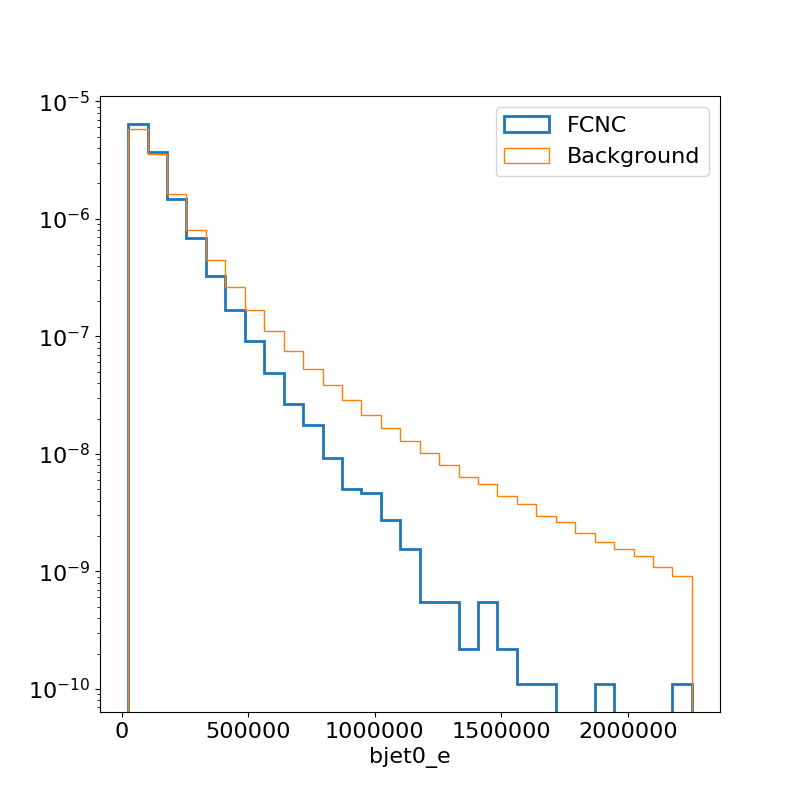
\includegraphics[width=.4\columnwidth]{../ThesisImages/SearchStrategy/varplots/bjet0_e.png}}\hfil
\subfloat[$\eta_b$]{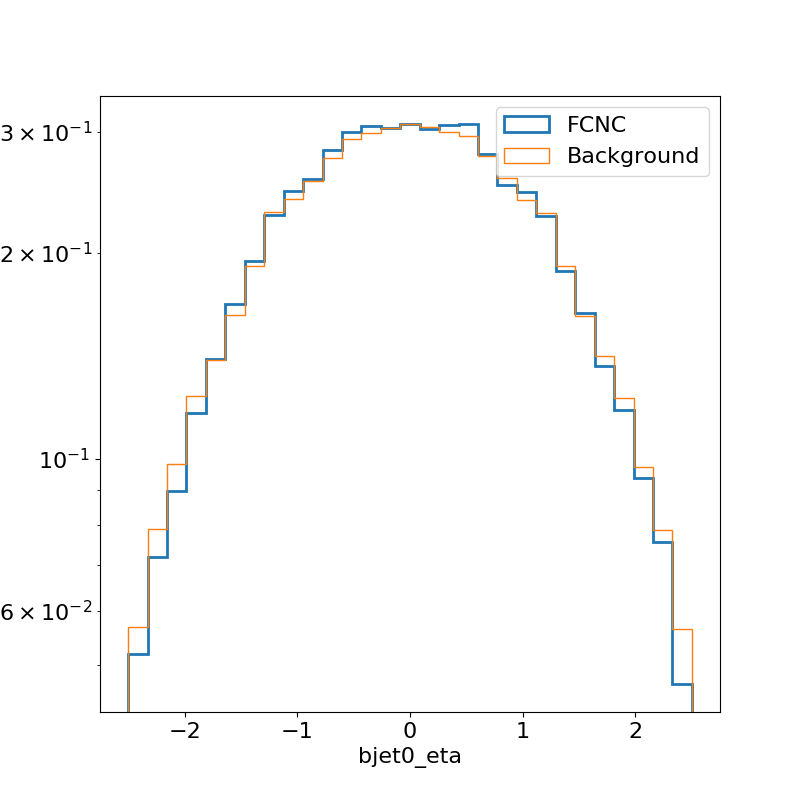
\includegraphics[width=.4\columnwidth]{../ThesisImages/SearchStrategy/varplots/bjet0_eta.png}}
\vspace{-4.5mm}
\subfloat[$\Delta R_{jb}$]{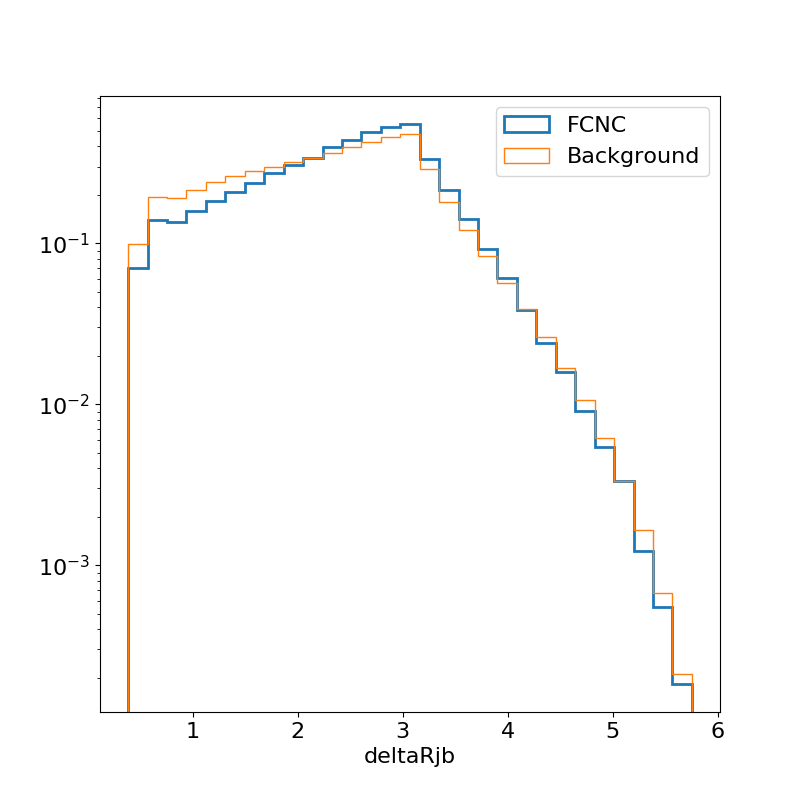
\includegraphics[width=.4\columnwidth]{../ThesisImages/SearchStrategy/varplots/deltaRjb.png}}\hfil
\subfloat[E (light jet)]{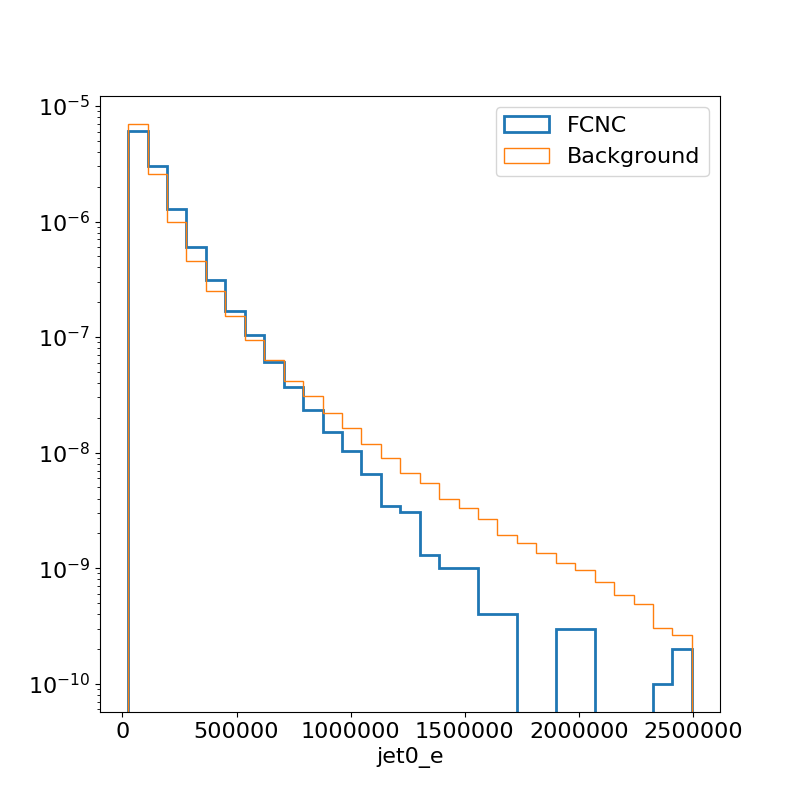
\includegraphics[width=.4\columnwidth]{../ThesisImages/SearchStrategy/varplots/jet0_e.png}}   
\vspace{-4.5mm}
\subfloat[light jet $\eta$]{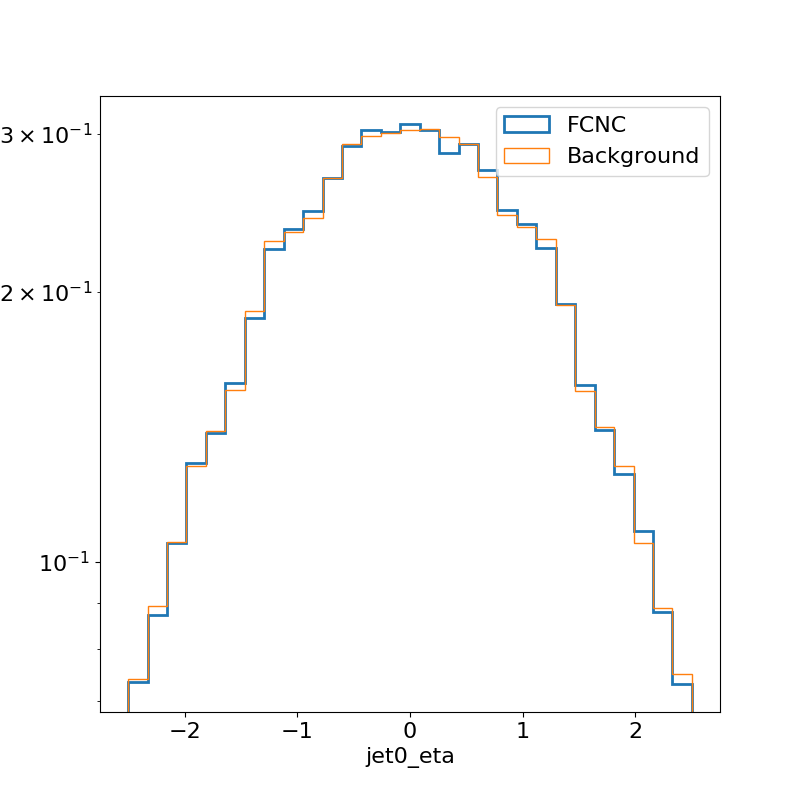
\includegraphics[width=.4\columnwidth]{../ThesisImages/SearchStrategy/varplots/jet0_eta.png}}\hfil
\subfloat[$\chi^2_\nu$]{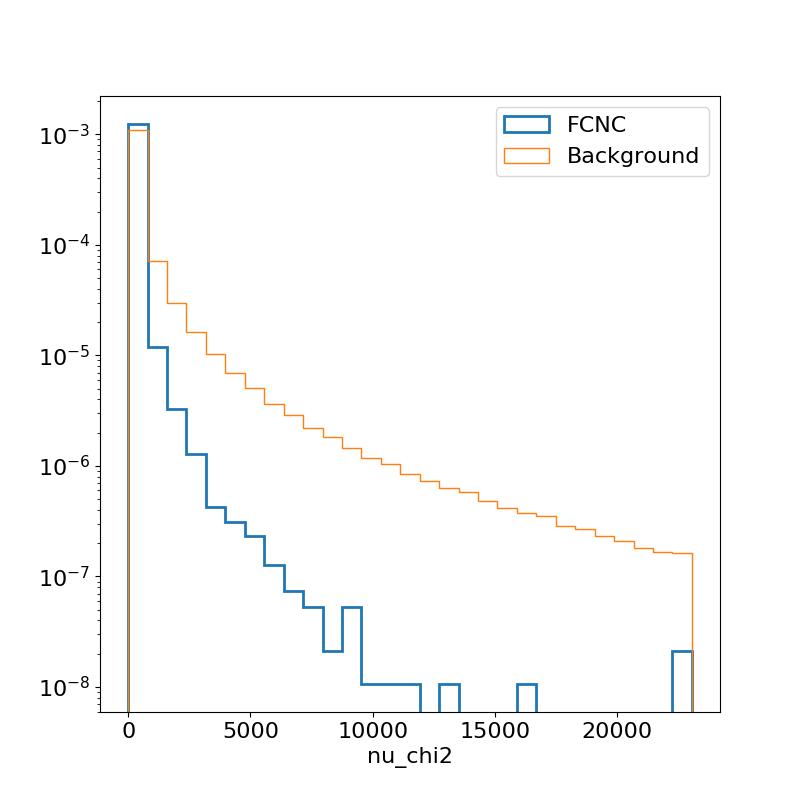
\includegraphics[width=.4\columnwidth]{../ThesisImages/SearchStrategy/varplots/nu_chi2.png}}
\caption{Normalized variables showing the shapes of neural network input variables for the $\mu$+jets channel: [E (bjet), $\eta_b$, $\Delta R_{jb}$, E (light jet), light jet $\eta$, and $\chi^2_\nu$ the total $\chi^2$ fit value  }
\label{fig:VarPlots4}
\end{figure}


\begin{figure}[h!]
\centering
\subfloat[lepton $p_T$]{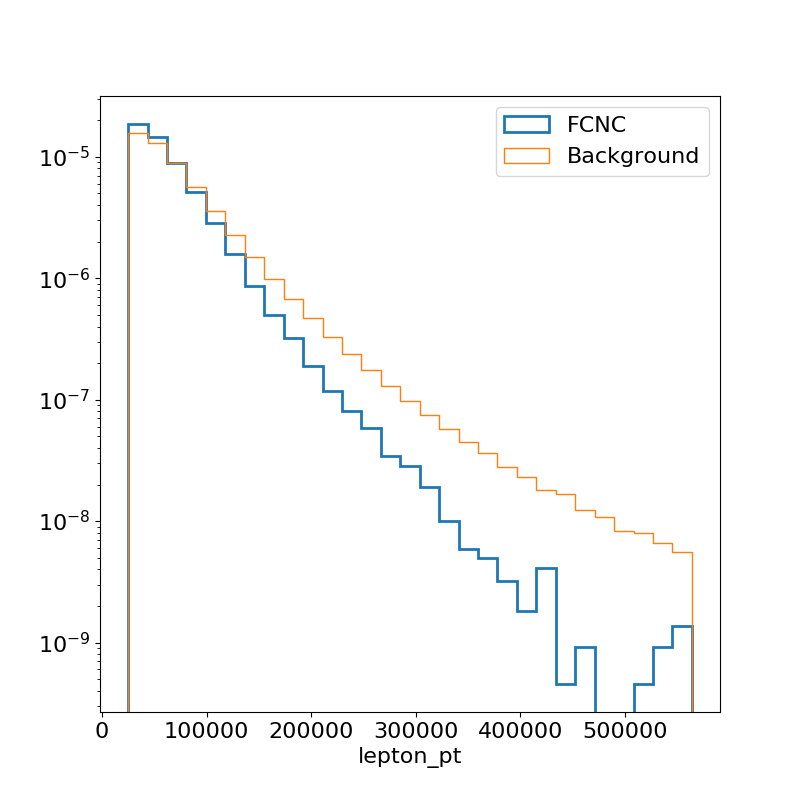
\includegraphics[width=.4\columnwidth]{../ThesisImages/SearchStrategy/varplots/lepton_pt}}\hfil
\subfloat[lepton $\eta$]{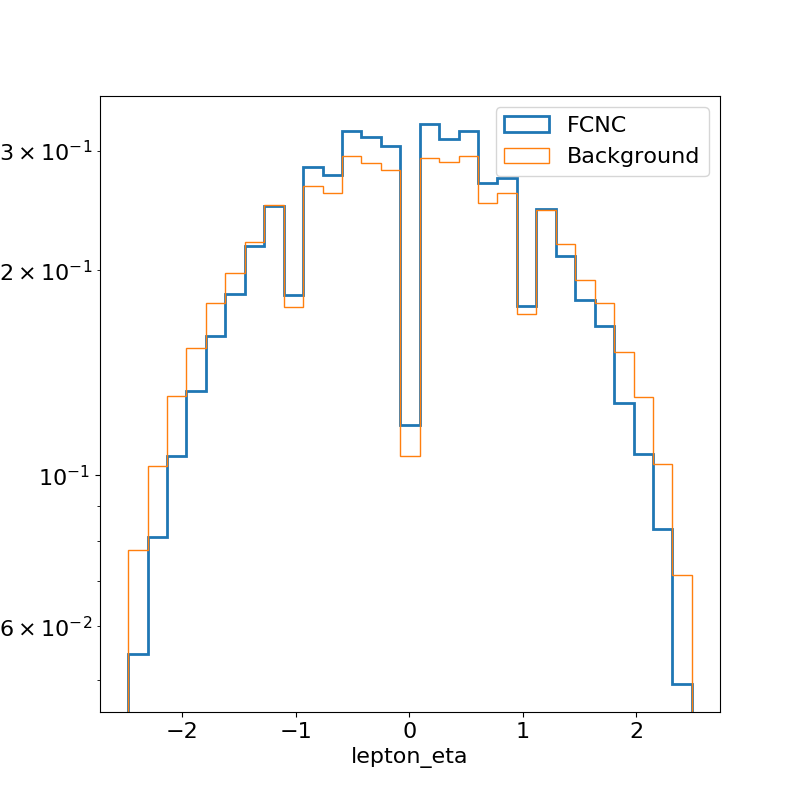
\includegraphics[width=.4\columnwidth]{../ThesisImages/SearchStrategy/varplots/lepton_eta.png}}
\vspace{-4.5mm}
\subfloat[lepton isolation]{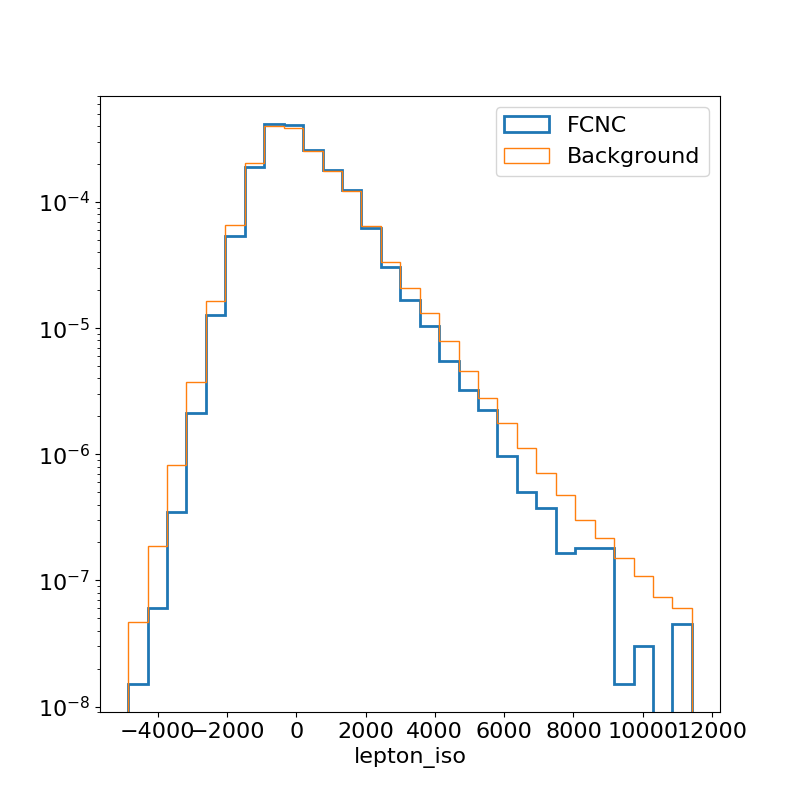
\includegraphics[width=.4\columnwidth]{../ThesisImages/SearchStrategy/varplots/lepton_iso.png}}\hfil
\subfloat[$\chi^2_{\text{bW}}$]{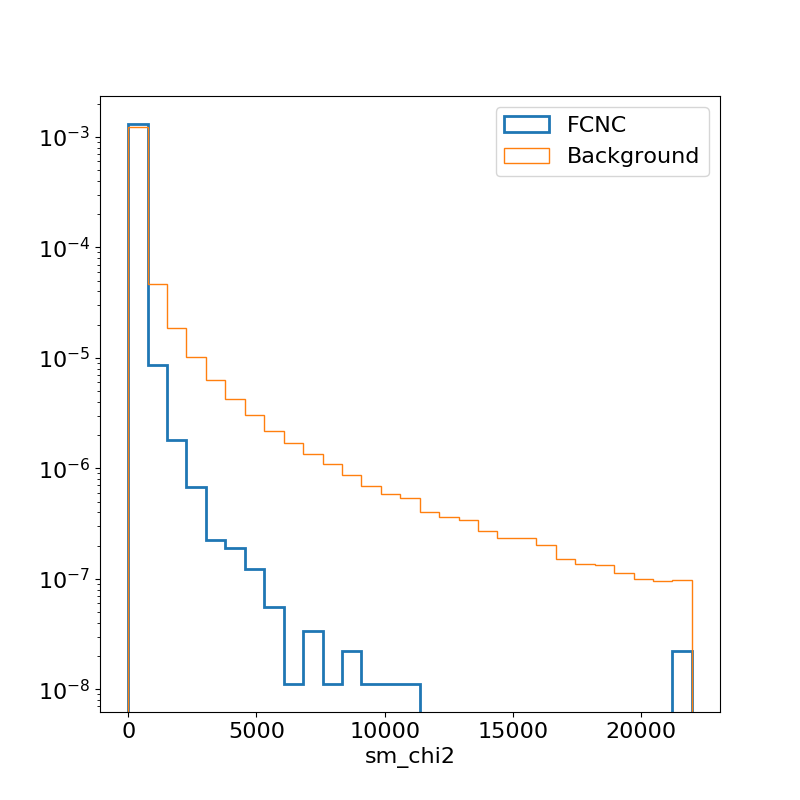
\includegraphics[width=.4\columnwidth]{../ThesisImages/SearchStrategy/varplots/sm_chi2.png}}   
\vspace{-4.5mm}
\subfloat[photon E]{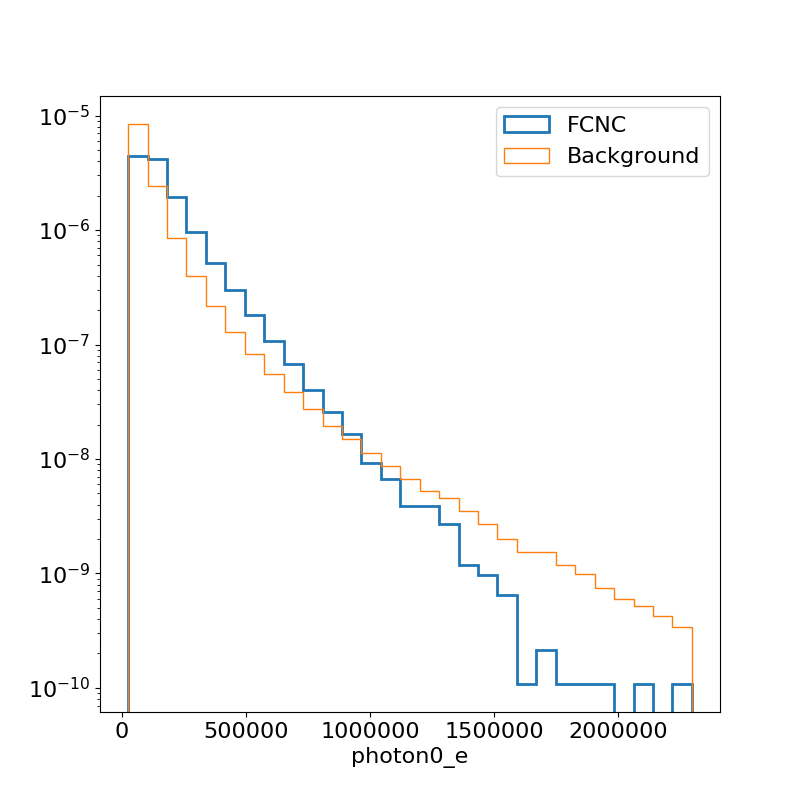
\includegraphics[width=.4\columnwidth]{../ThesisImages/SearchStrategy/varplots/photon0_e.png}}\hfil
\subfloat[photon $\eta$]{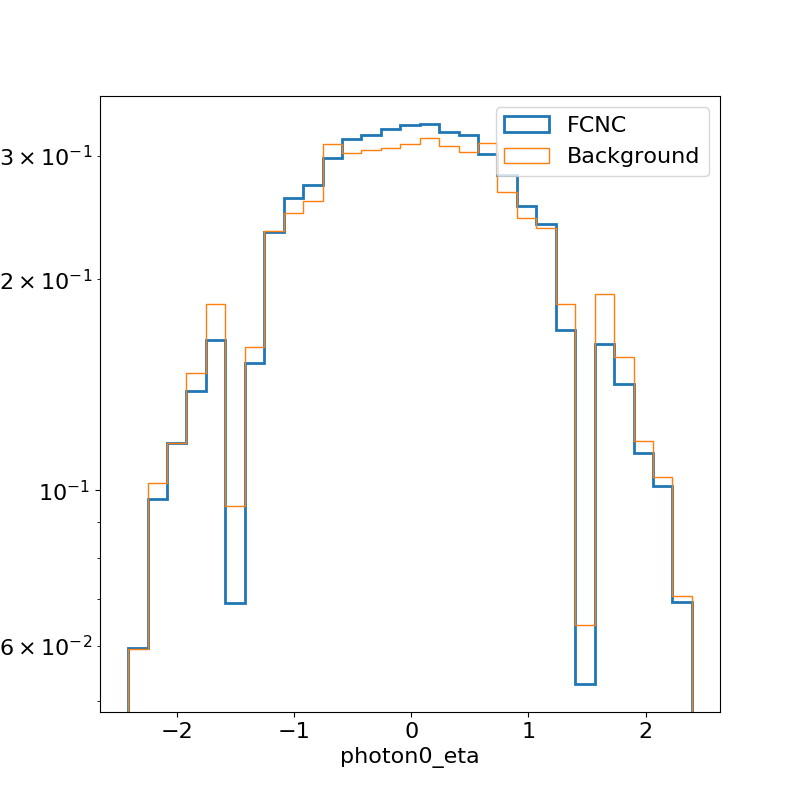
\includegraphics[width=.4\columnwidth]{../ThesisImages/SearchStrategy/varplots/photon0_eta.png}}
\caption{Normalized variables showing the shapes of neural network input variables for the $\mu$+jets channel: [lepton $p_T$, lepton $\eta$, lepton isolation , $chi^2_{\text{SM}}$ the bW$\chi^2$ value from neutrino reconstrucion ,photon E, and photon $\eta$.  }
\label{fig:VarPlots5}
\end{figure}

\section{Shape Comparison Plots: $e$+jets channel}

\begin{figure}[h!]
\centering
\subfloat[$\Delta R_{l \gamma}$]{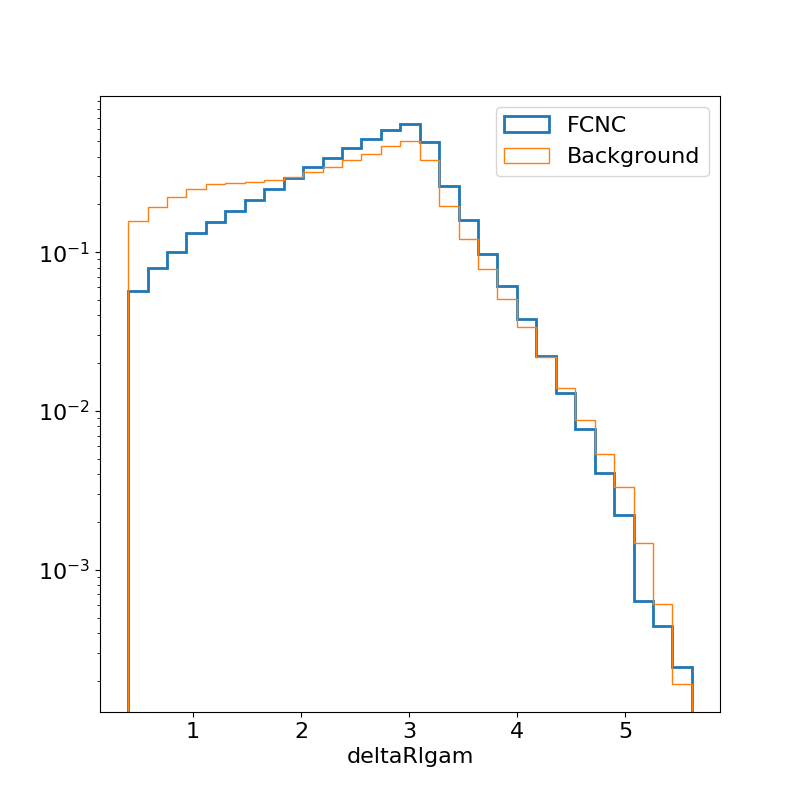
\includegraphics[width=.4\columnwidth]{../ThesisImages/SearchStrategy/varplots/ejets/deltaRlgam.png}}\hfil
\subfloat[E (lepton)]{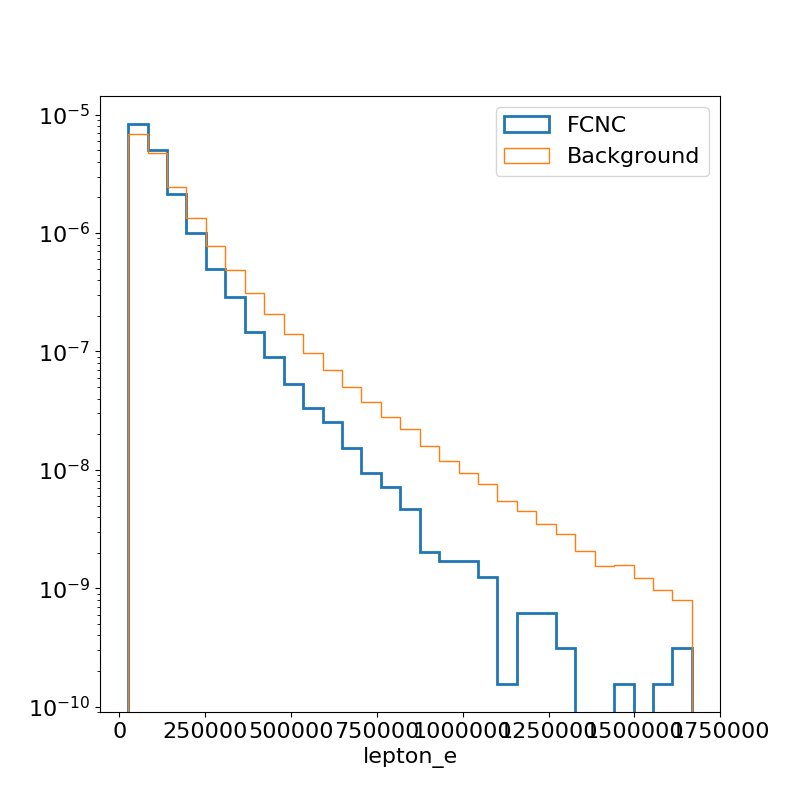
\includegraphics[width=.4\columnwidth]{../ThesisImages/SearchStrategy/varplots/ejets/lepton_e.png}}
\vspace{-4.5mm}
\subfloat[$\slashed{E}_T  $]{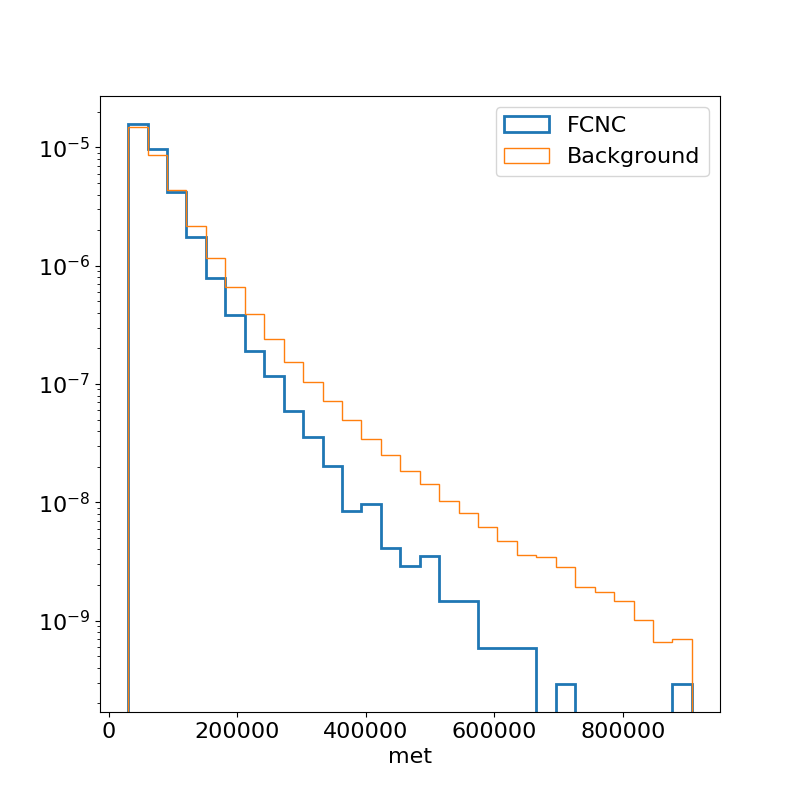
\includegraphics[width=.4\columnwidth]{../ThesisImages/SearchStrategy/varplots/ejets/met.png}}\hfil
\subfloat[$p_T (b)$ ]{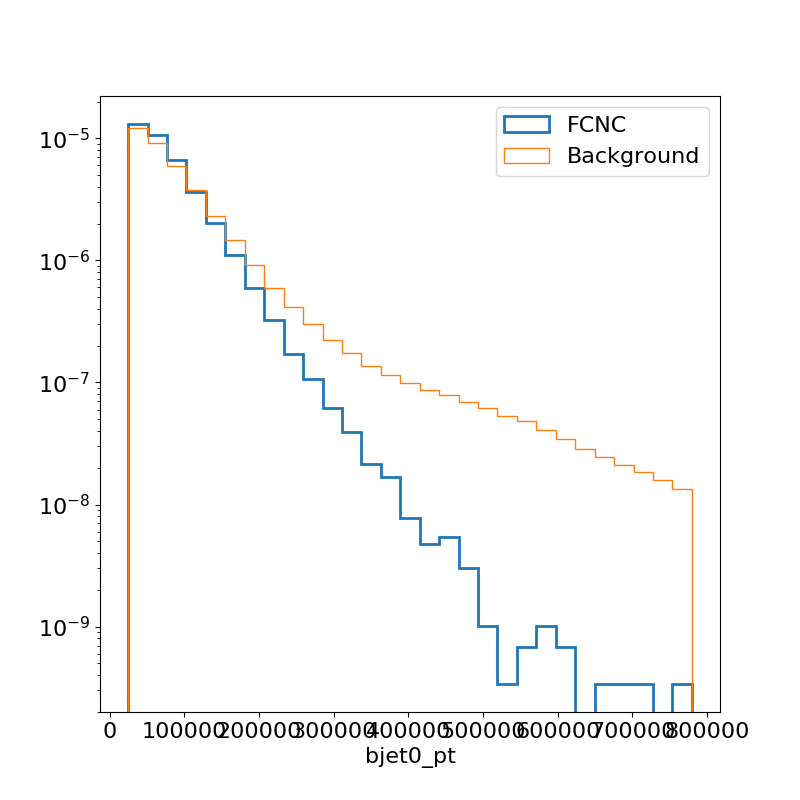
\includegraphics[width=.4\columnwidth]{../ThesisImages/SearchStrategy/varplots/ejets/bjet0_pt.png}}   
\caption{Normalized variables showing the shapes of neural network input variables for the $e$+jets channel: $\Delta R_{l \gamma}$, E (lepton), $\slashed{E}_T  $, and $p_T (b)$}
\label{fig:VarPlotsej3}
\end{figure}

\begin{figure}[h!]
\centering
\subfloat[$\gamma_{iso}$ topo$E_{T}$cone40]{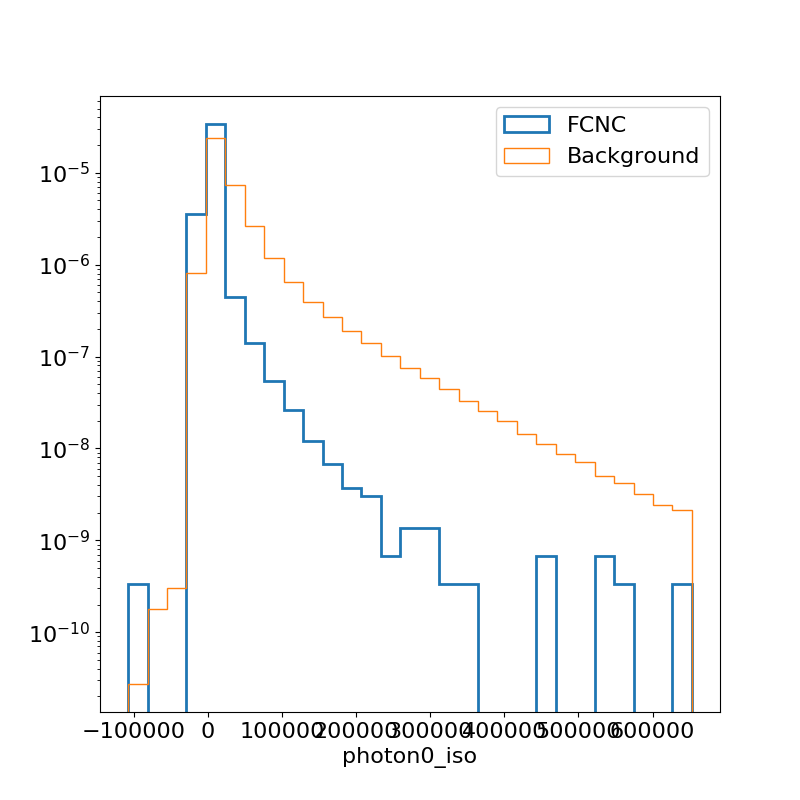
\includegraphics[width=.4\columnwidth]{../ThesisImages/SearchStrategy/varplots/ejets/photon0_iso.png}}\hfil
\subfloat[$\gamma_{p_T}$]{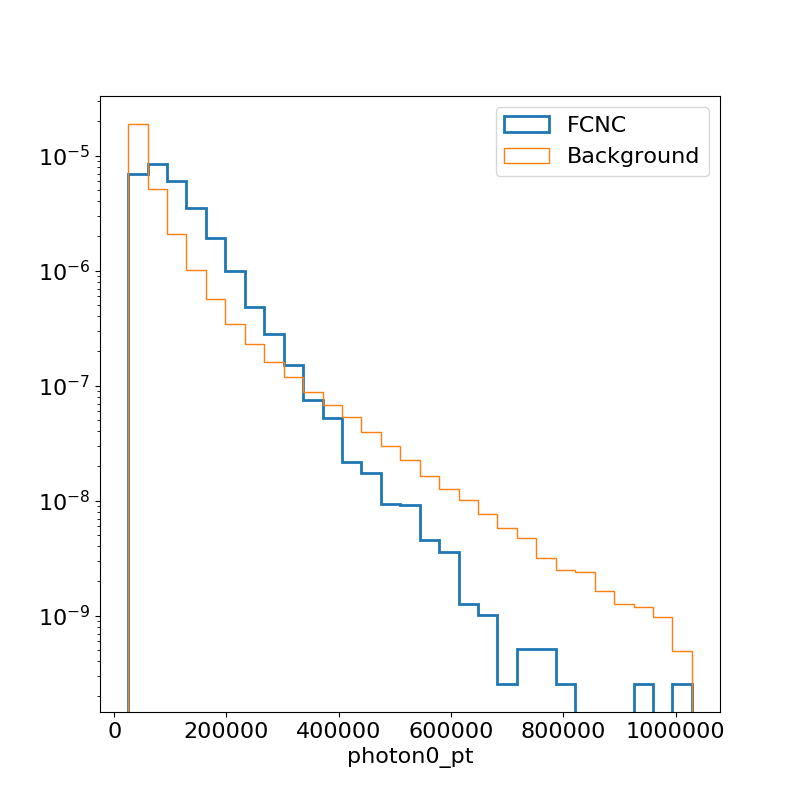
\includegraphics[width=.4\columnwidth]{../ThesisImages/SearchStrategy/varplots/ejets/photon0_pt.png}}
\vspace{-4.5mm}
\subfloat[$m_{q \gamma}$]{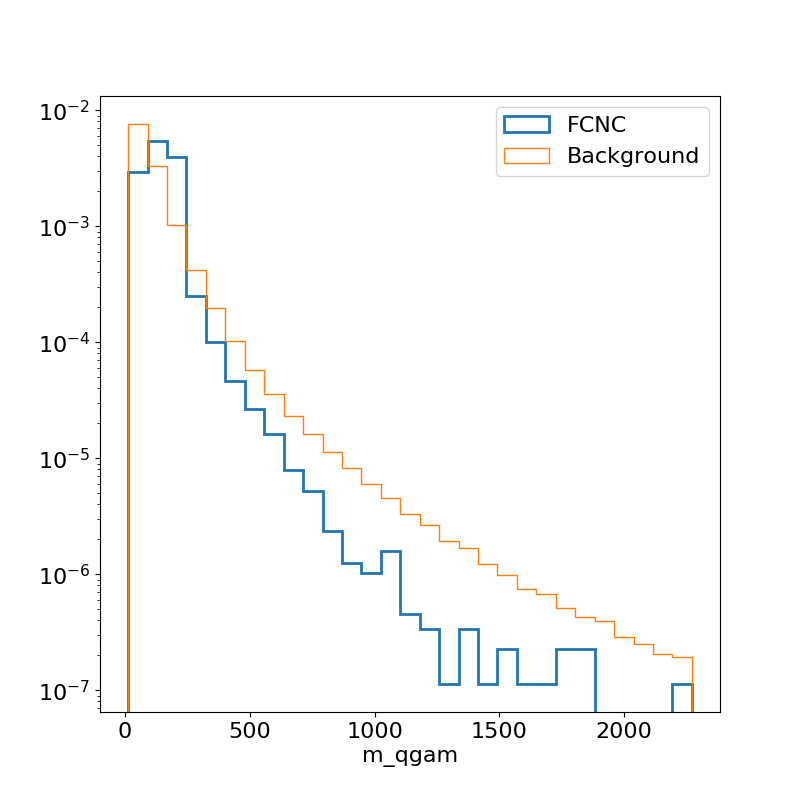
\includegraphics[width=.4\columnwidth]{../ThesisImages/SearchStrategy/varplots/ejets/m_qgam.png}}\hfil
\subfloat[$m_{l \gamma}$]{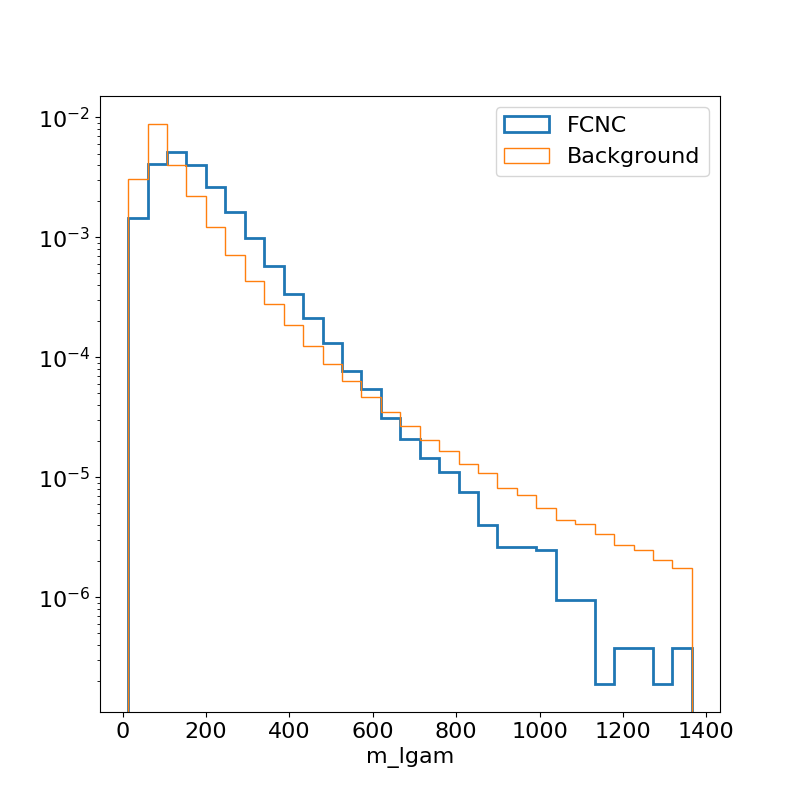
\includegraphics[width=.4\columnwidth]{../ThesisImages/SearchStrategy/varplots/ejets/m_lgam.png}}   
\vspace{-4.5mm}
\subfloat[$m_{bW}$]{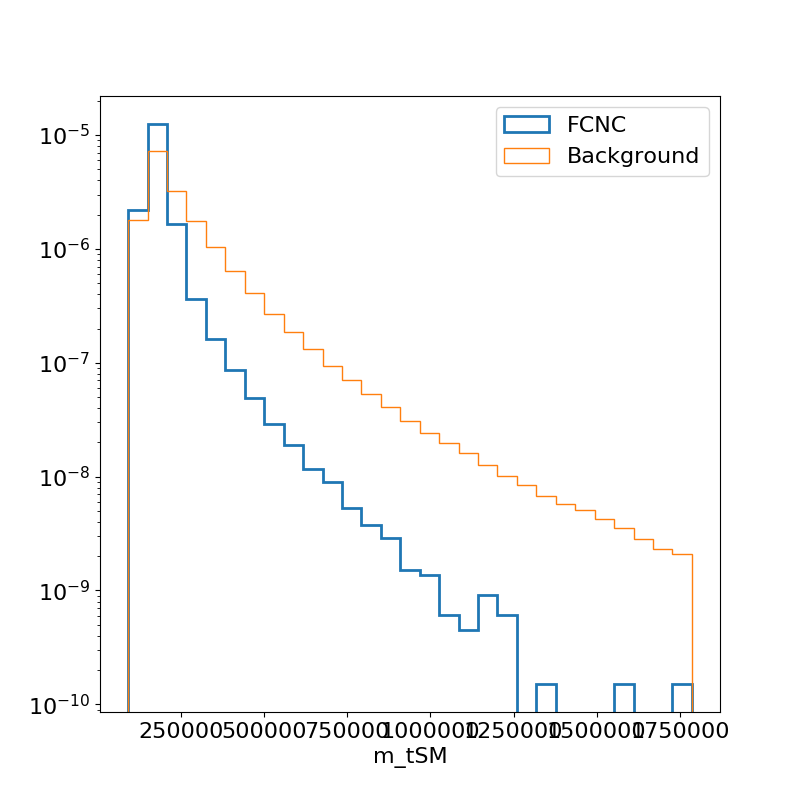
\includegraphics[width=.4\columnwidth]{../ThesisImages/SearchStrategy/varplots/ejets/m_tSM.png}}\hfil
\subfloat[$\Delta R_{j\gamma}$]{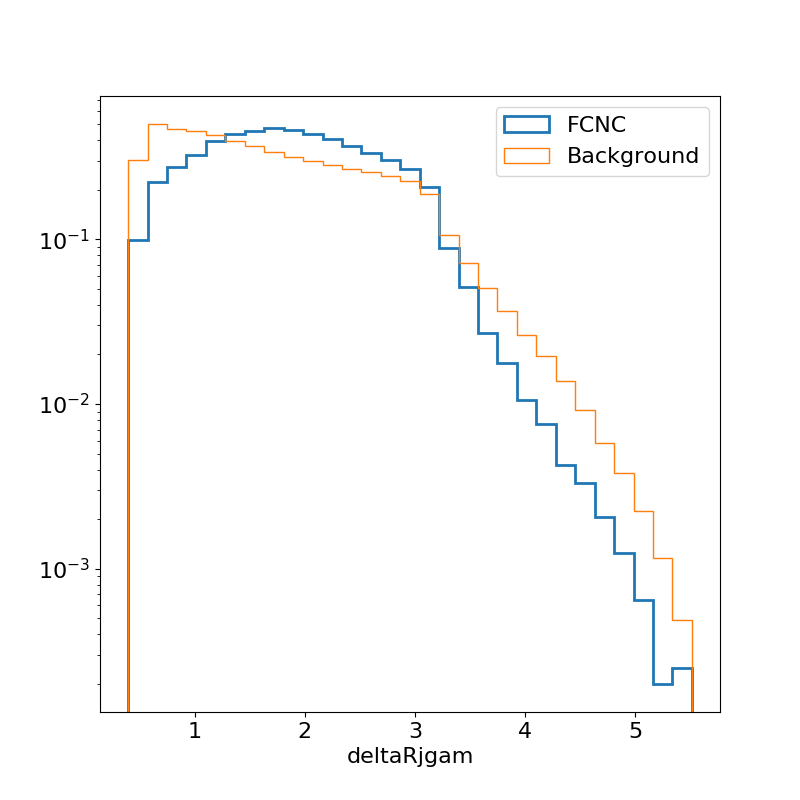
\includegraphics[width=.4\columnwidth]{../ThesisImages/SearchStrategy/varplots/ejets/deltaRjgam.png}}
\caption{Normalized variables showing the shapes of neural network input variables for the $e$+jets channel: $\gamma_{iso}$ topo$E_{T}$cone40, $\gamma_{p_T}$, $m_{q \gamma}$, $m_{l \gamma}$, $m_{bW}$, and $\Delta R_{j\gamma}$ }
\label{fig:VarPlotsej1}
\end{figure}

\begin{figure}[h!]
\centering
\subfloat[$\Delta R_{b l}$]{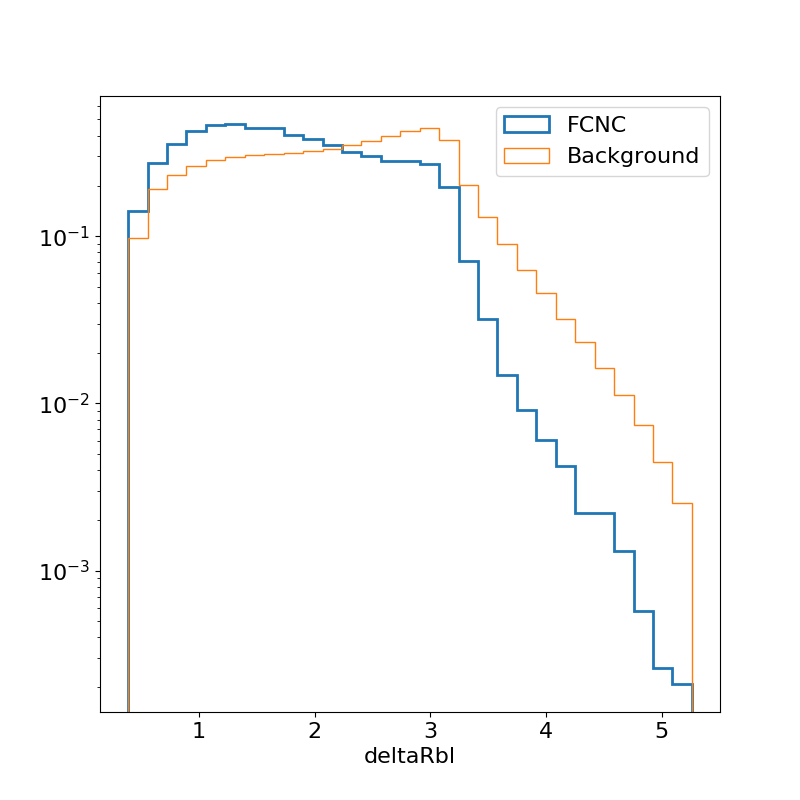
\includegraphics[width=.4\columnwidth]{../ThesisImages/SearchStrategy/varplots/ejets/deltaRbl.png}}\hfil
\subfloat[$m_{T}^{W}$ ]{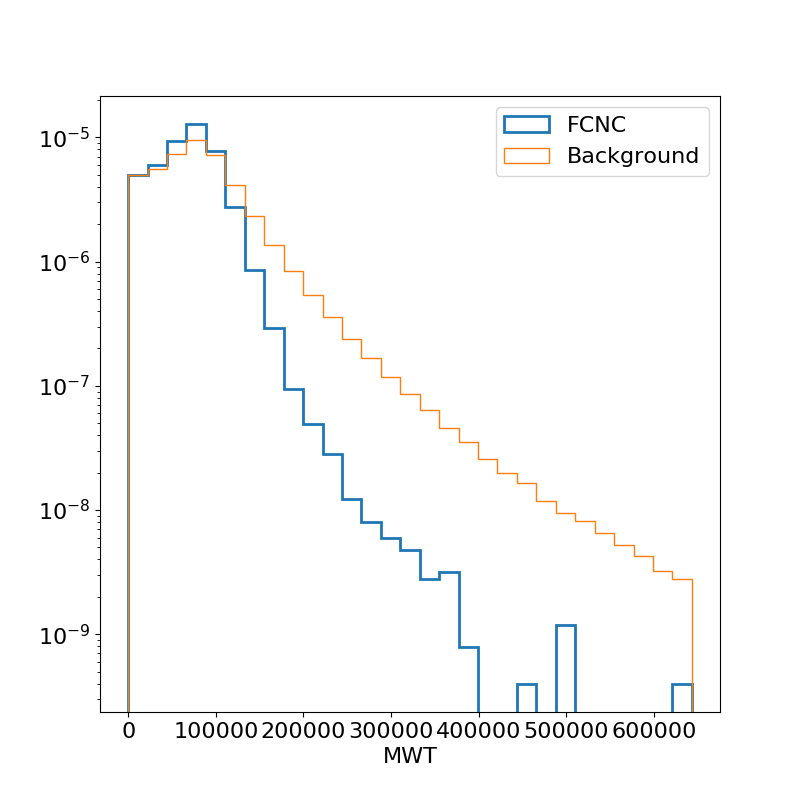
\includegraphics[width=.4\columnwidth]{../ThesisImages/SearchStrategy/varplots/ejets/MWT.png}}
\vspace{-4.5mm}
\subfloat[$S_T$]{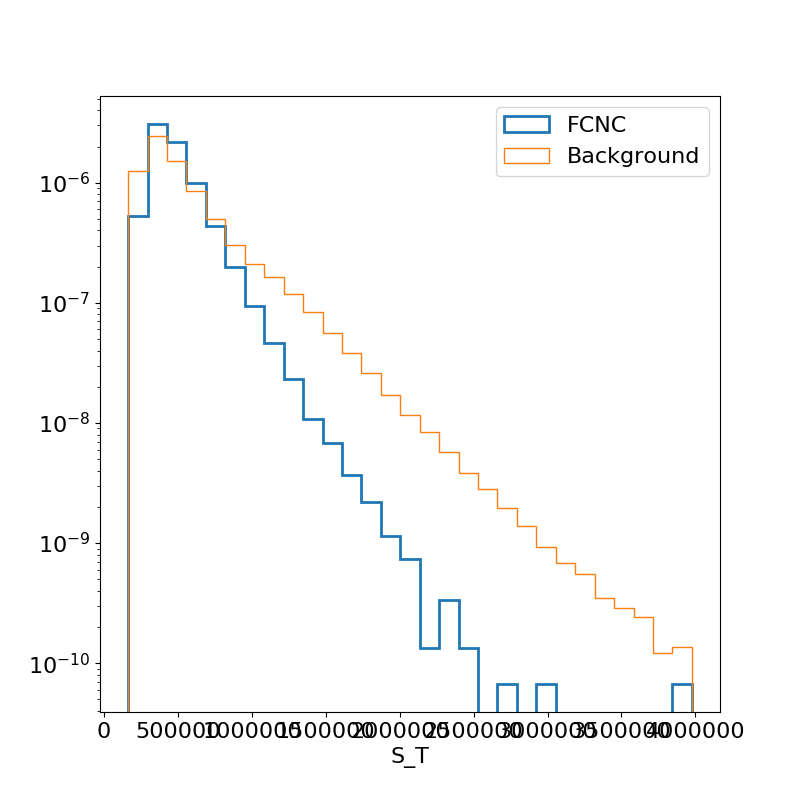
\includegraphics[width=.4\columnwidth]{../ThesisImages/SearchStrategy/varplots/ejets/S_T.png}}\hfil
\subfloat[$n_{\text{jets}}$]{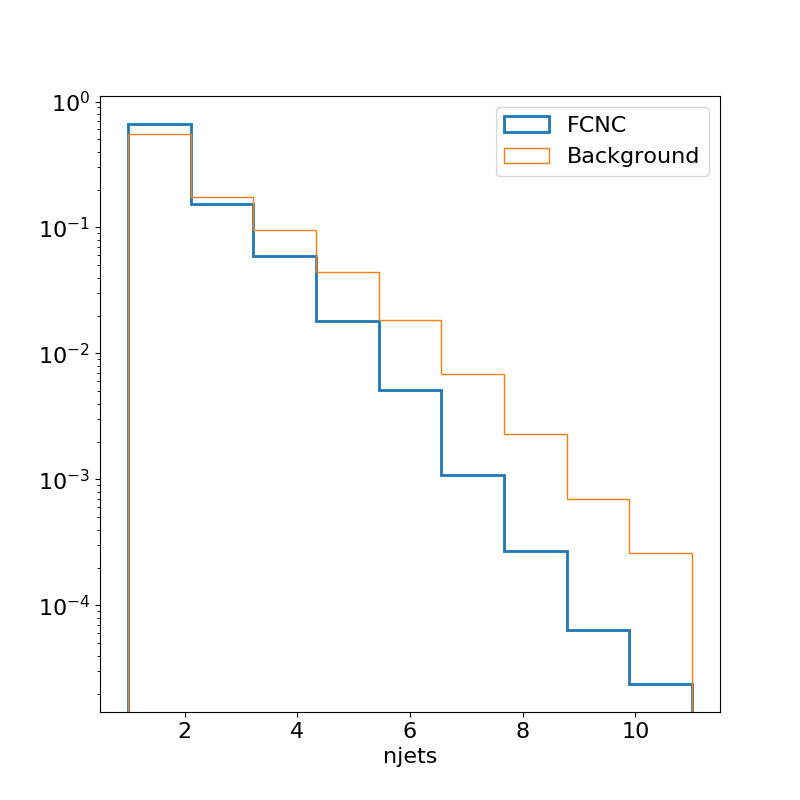
\includegraphics[width=.4\columnwidth]{../ThesisImages/SearchStrategy/varplots/ejets/njets.png}}   
\vspace{-4.5mm}
\subfloat[$\chi^{2}_{W}$]{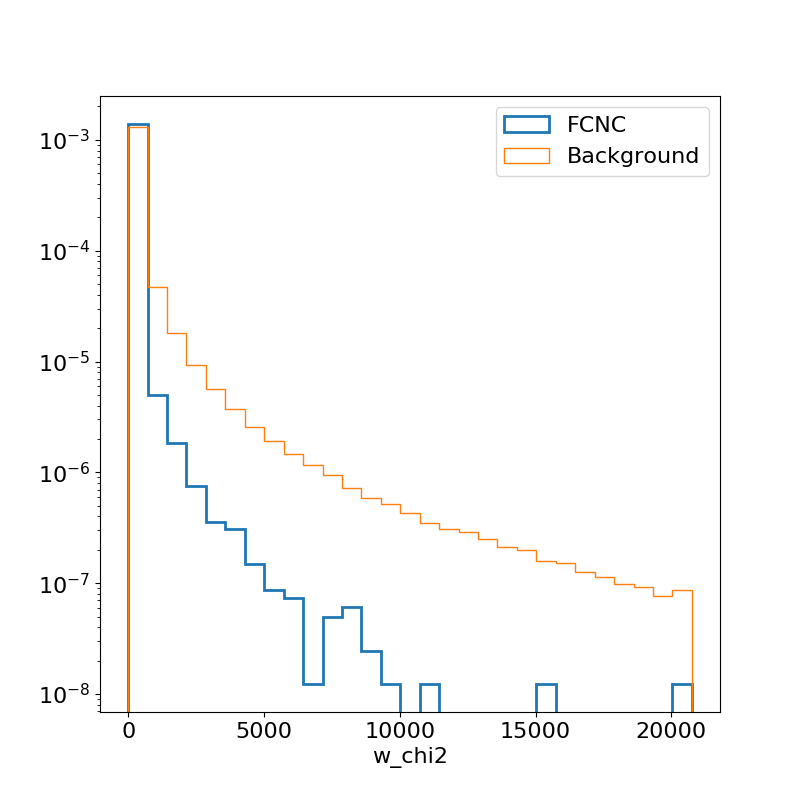
\includegraphics[width=.4\columnwidth]{../ThesisImages/SearchStrategy/varplots/ejets/w_chi2.png}}\hfil
\subfloat[$p_T (q)$]{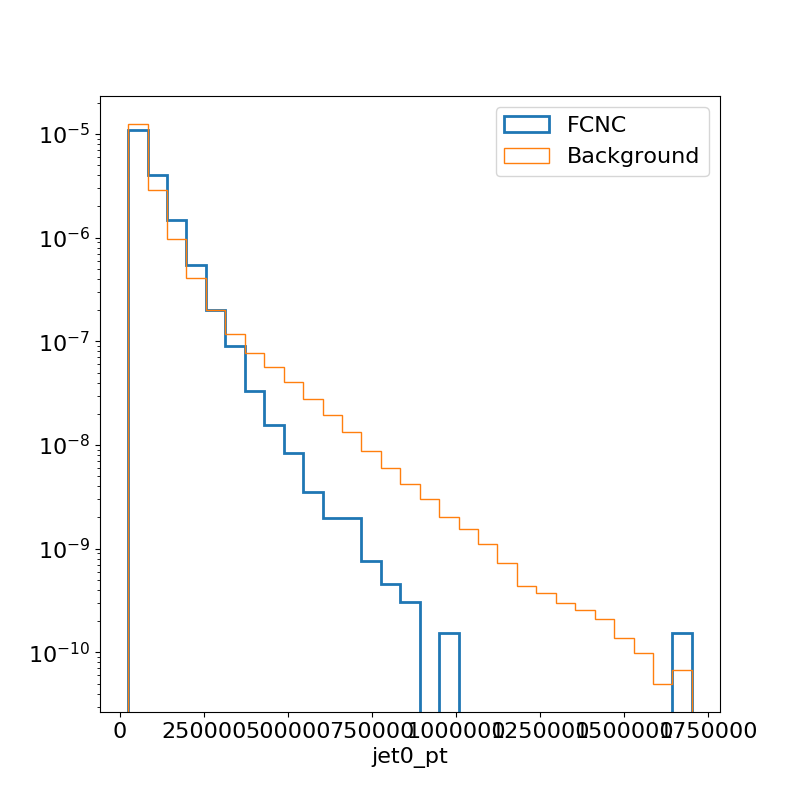
\includegraphics[width=.4\columnwidth]{../ThesisImages/SearchStrategy/varplots/ejets/jet0_pt.png}}
\caption{Normalized variables showing the shapes of neural network input variables for the $e$+jets channel: $\Delta R_{b l}$, $m_{T}^{W}$ , $S_T$, $n_{\text{jets}}$, $\chi^{2}_{W}$, and $p_T (q)$}
\label{fig:VarPlotsej2}
\end{figure}


\begin{figure}[h!]
\centering
\subfloat[E (bjet)]{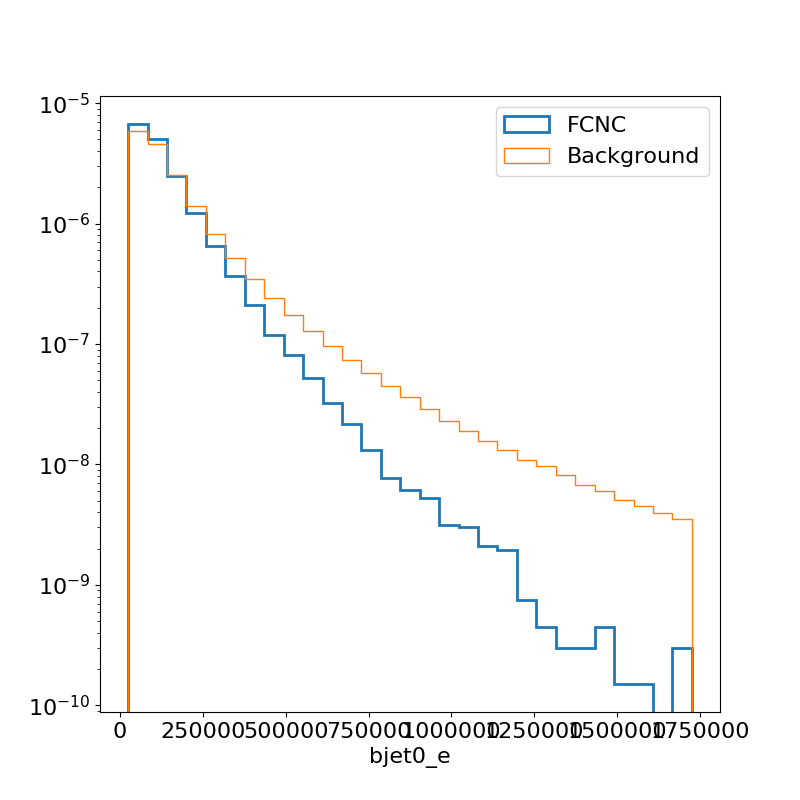
\includegraphics[width=.4\columnwidth]{../ThesisImages/SearchStrategy/varplots/ejets/bjet0_e.png}}\hfil
\subfloat[$\eta_b$]{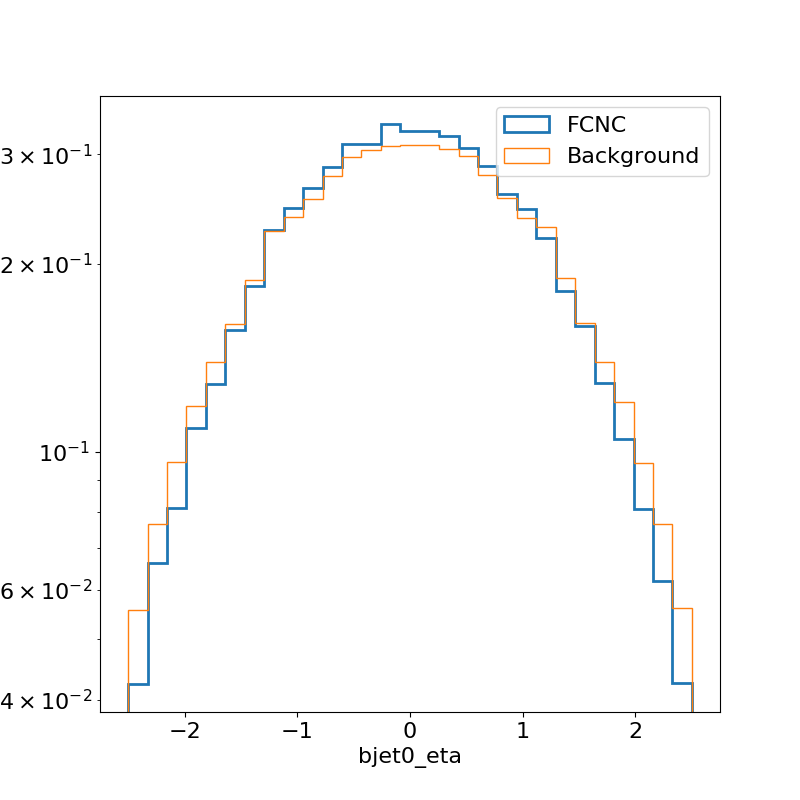
\includegraphics[width=.4\columnwidth]{../ThesisImages/SearchStrategy/varplots/ejets/bjet0_eta.png}}
\vspace{-4.5mm}
\subfloat[$\Delta R_{jb}$]{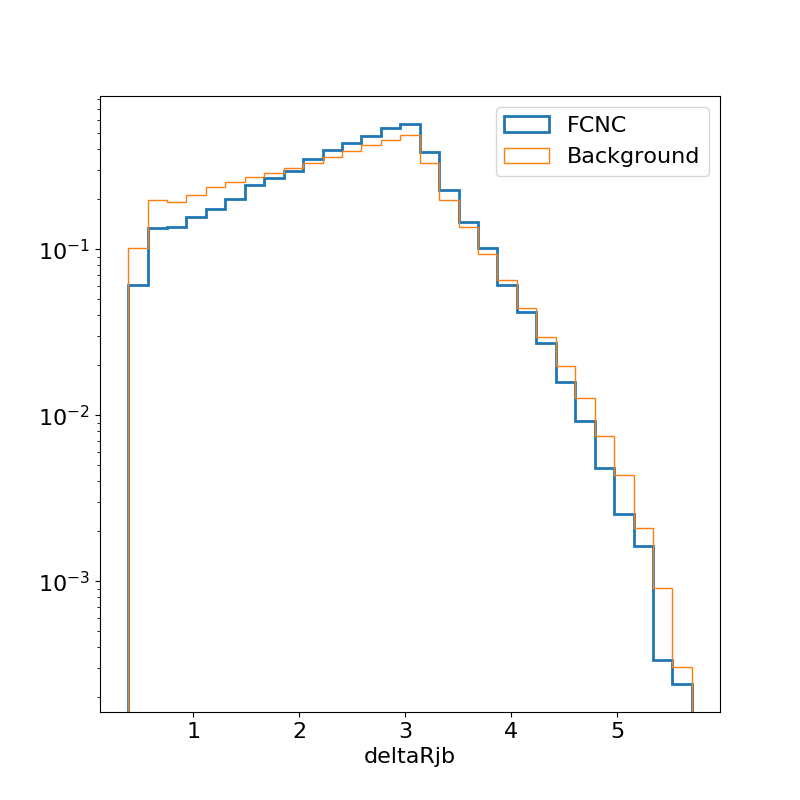
\includegraphics[width=.4\columnwidth]{../ThesisImages/SearchStrategy/varplots/ejets/deltaRjb.png}}\hfil
\subfloat[E (light jet)]{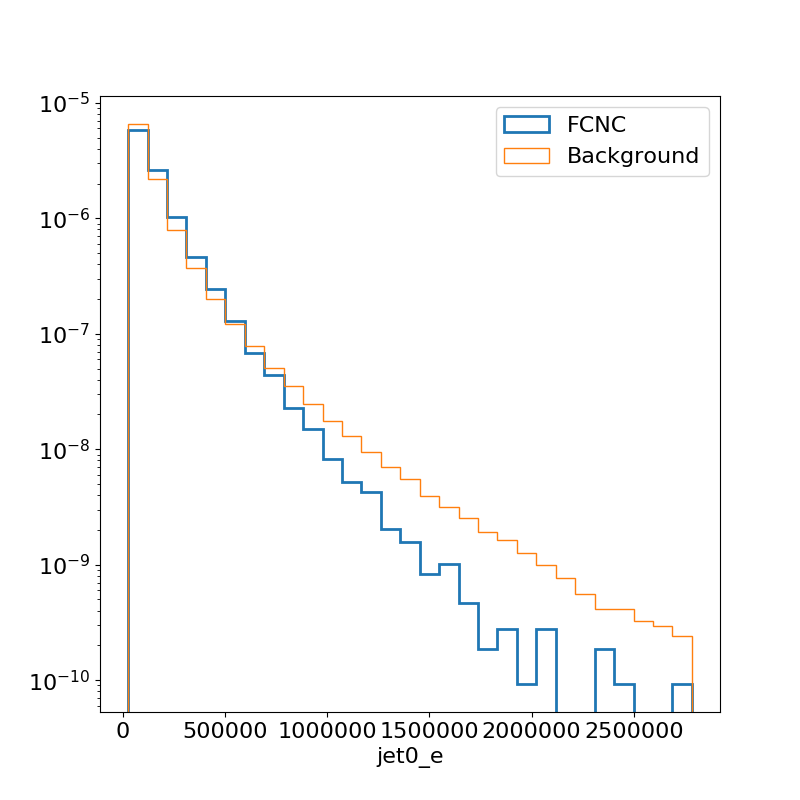
\includegraphics[width=.4\columnwidth]{../ThesisImages/SearchStrategy/varplots/ejets/jet0_e.png}}   
\vspace{-4.5mm}
\subfloat[light jet $\eta$]{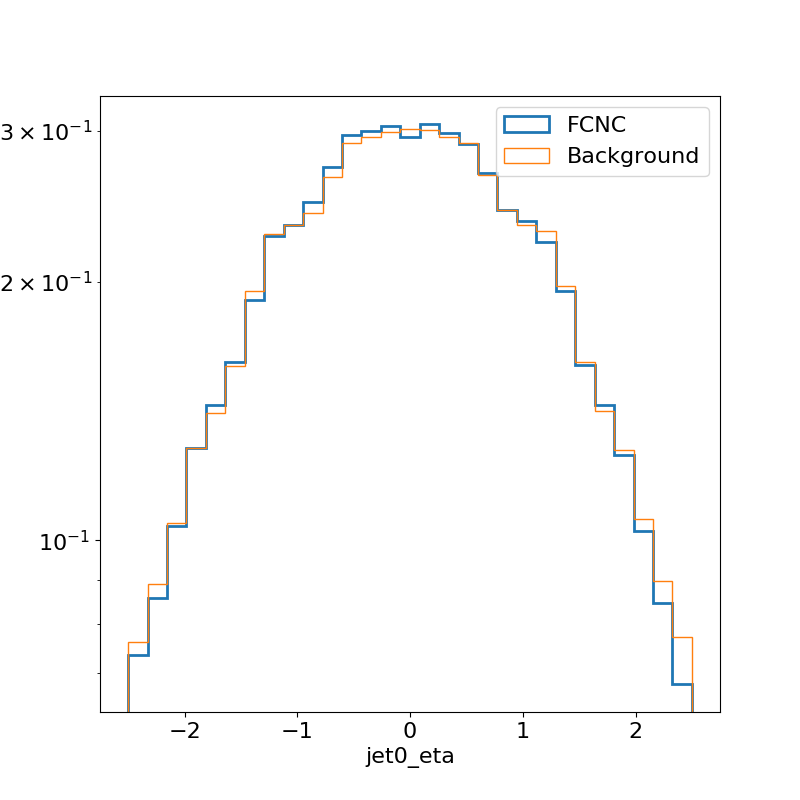
\includegraphics[width=.4\columnwidth]{../ThesisImages/SearchStrategy/varplots/ejets/jet0_eta.png}}\hfil
\subfloat[$\chi^2_\nu$]{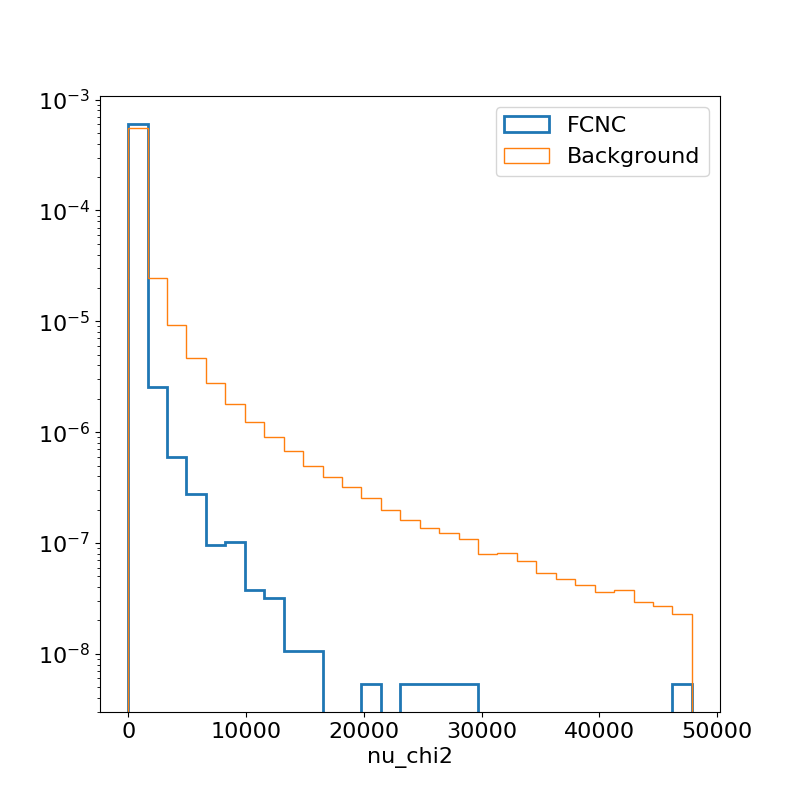
\includegraphics[width=.4\columnwidth]{../ThesisImages/SearchStrategy/varplots/ejets/nu_chi2.png}}
\caption{Normalized variables showing the shapes of neural network input variables for the $e$+jets channel: [E (bjet), $\eta_b$, $\Delta R_{jb}$, E (light jet), light jet $\eta$, and $\chi^2_\nu$ the total $\chi^2$ fit value  }
\label{fig:VarPlotsej4}
\end{figure}


\begin{figure}[h!]
\centering
\subfloat[lepton $p_T$]{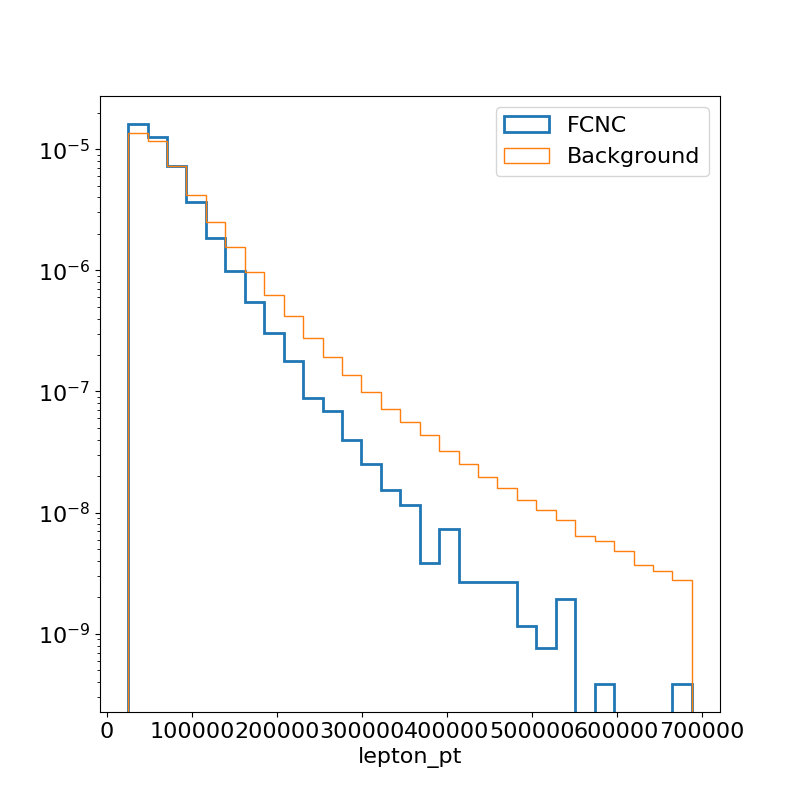
\includegraphics[width=.4\columnwidth]{../ThesisImages/SearchStrategy/varplots/ejets/lepton_pt}}\hfil
\subfloat[lepton $\eta$]{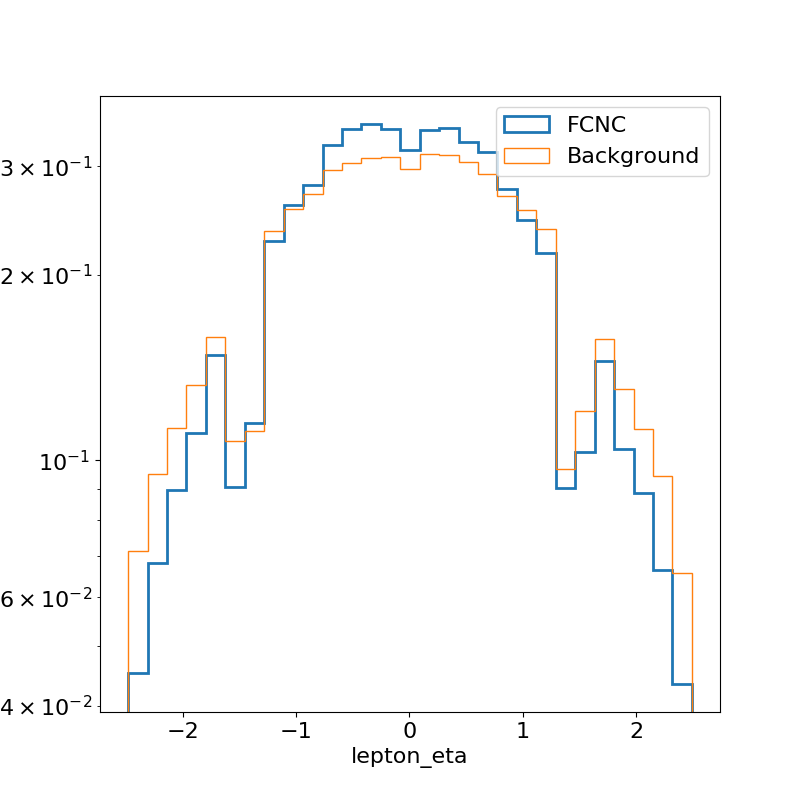
\includegraphics[width=.4\columnwidth]{../ThesisImages/SearchStrategy/varplots/ejets/lepton_eta.png}}
\vspace{-4.5mm}
\subfloat[lepton isolation]{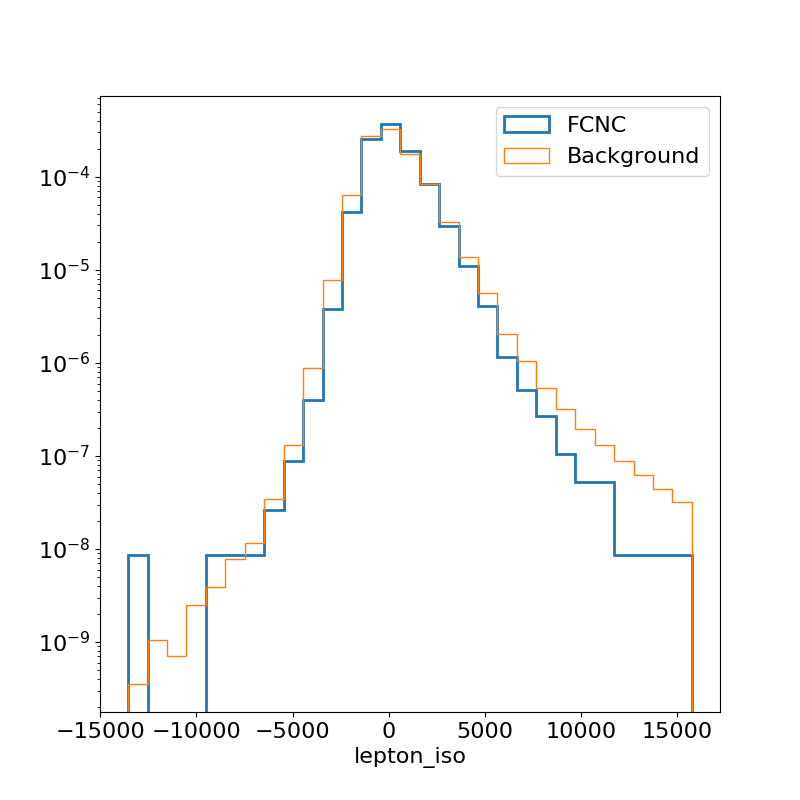
\includegraphics[width=.4\columnwidth]{../ThesisImages/SearchStrategy/varplots/ejets/lepton_iso.png}}\hfil
\subfloat[$\chi^2_{\text{bW}}$]{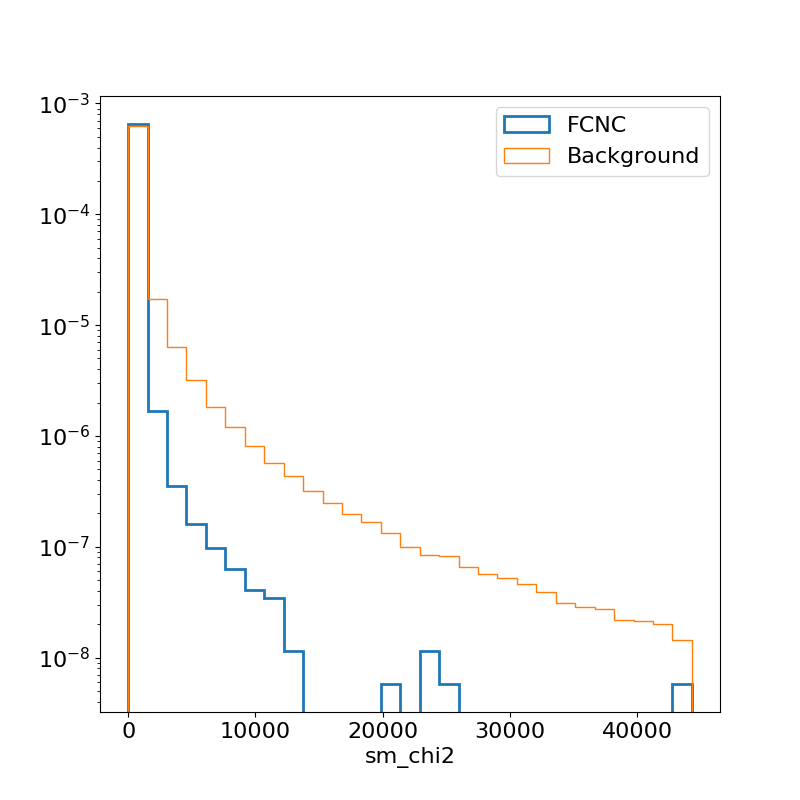
\includegraphics[width=.4\columnwidth]{../ThesisImages/SearchStrategy/varplots/ejets/sm_chi2.png}}   
\vspace{-4.5mm}
\subfloat[photon E]{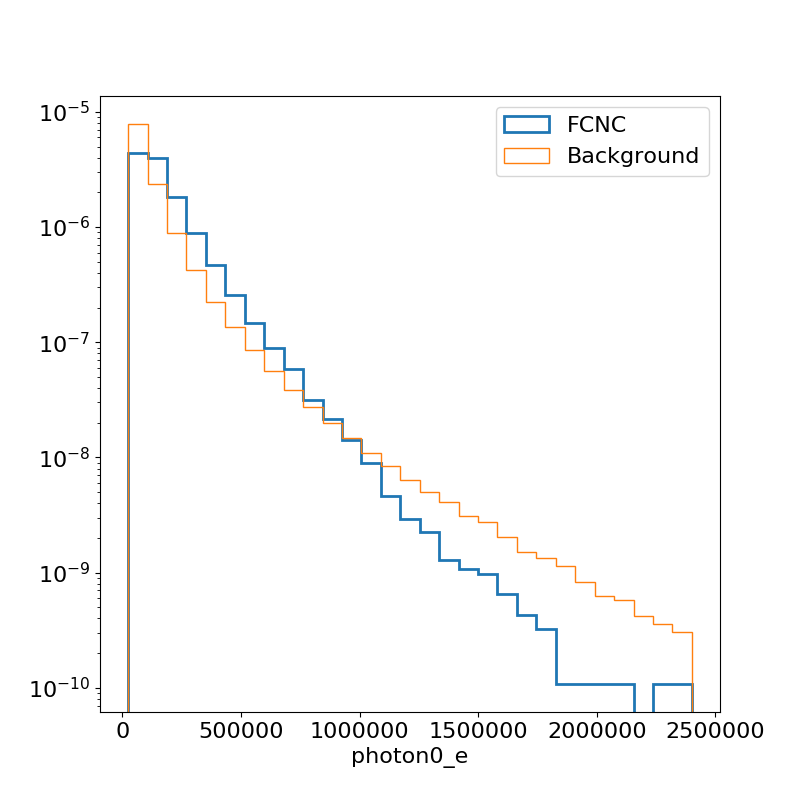
\includegraphics[width=.4\columnwidth]{../ThesisImages/SearchStrategy/varplots/ejets/photon0_e.png}}\hfil
\subfloat[photon $\eta$]{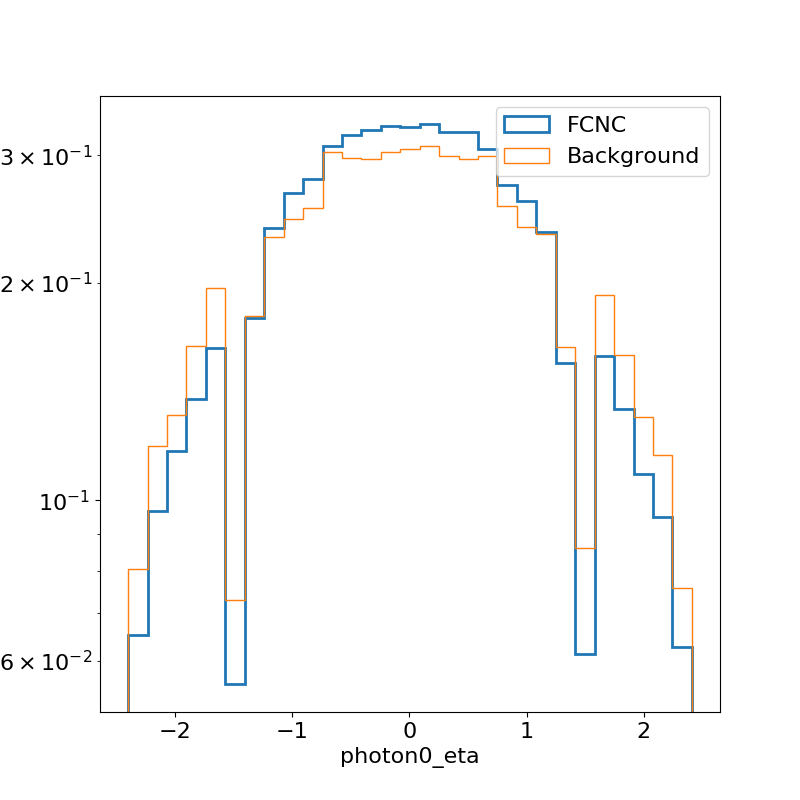
\includegraphics[width=.4\columnwidth]{../ThesisImages/SearchStrategy/varplots/ejets/photon0_eta.png}}
\caption{Normalized variables showing the shapes of neural network input variables for the $e$+jets channel: [lepton $p_T$, lepton $\eta$, lepton isolation , $chi^2_{\text{SM}}$ the bW$\chi^2$ value from neutrino reconstrucion, photon E, and photon $\eta$.  }
\label{fig:VarPlotsej5}
\end{figure}

